\chapter{\label{ch:2-CNNs}Deep learning methods and their applications for IACTs}
\minitoc
\begin{abstract}
    Deep learning analysis methods based upon CNNs are becoming increasingly widely utilised throughout the physical sciences. In this chapter we explore the basic properties of such methods, before reviewing past and concurrent work on utilising these methods with IACT data. We then go on to explore the known issues with applying these methods to IACT data in depth.
\end{abstract}

\section{Introduction}

Machine learning has been critical to the operation of the current generation of IACTs, H.E.S.S., MAGIC and VERITAS. As explored in Chapter \ref{ch:1-intro}, BDT-based methods used currently have offered a significant sensitivity improvement over conventional Hillas parameter cuts alone. However, when dealing with a new generation of IACT cameras with improved pixel density and timing precision, these BDT methods have notable shortcoming. This is that they do not take account of all the image and timing information available to them. This is a very similar situation to IACT astronomy in the early 2000s, as the construction of the current generation of IACTs with larger cameras necessitated the development of BDT and template fitting techniques. As such, the machine learning task force in CTA was set up to investigate whether it is possible to obtain a sensitivity improvement for CTA by using new deep learning techniques. At the same time, deep learning is a very rapidly advancing field, new models and methods of handling data are constantly becoming available (see for example \cite{adithesis} \cite{chebnet}), but these new methods must be adapted and tempered for IACT analysis. In this chapter, we explore the current state of the art in machine learning methods in greater depth, before going on to explore past work on implementing newly available deep learning techniques for IACT data, and some of the problems that have already been found. 

New deep learning methods, which are neural network methods with many layers, or equivalently a high degree of feature abstraction, are frequently associated with `AI'. Despite this, true emergent AI that can interpret universal input data and formulate meaningful responses remains science fiction, with no serious research currently being performed \cite{emergent}. In practice, most supervised deep learning techniques are simply an advanced form of pattern recognition, with weights being adjusted to provide known responses to known training data. When exposed to new data outside of their original training data sample these methods often run into difficulties, an area of computer science research referred to as `Domain Adaptation' \cite{wilson}. We will begin to encounter such difficulties in Chapter \ref{ch:4-VERITASRealData}.

\subsection{Types of Machine Learning}
Before addressing substantially the novel elements of this thesis, it is necessary for us to introduce a number of basic concepts and terms. \textbf{Supervised Machine Learning} refers to the areas of automated pattern recognition whereby labelled \textbf{Training Data} exists such that a configurable function can be optimised to map an input to a desired output. \textbf{Unsupervised Machine Learning} refers to the field of machine learning research where the underlying relationship between input and output is not known a-priori, such as in the case of clustering analysis. Whilst this can have some analysis uses in $\gamma$-ray astronomy \cite{tomthesis}, such as source detection, it is not the focus of the work in this thesis. In our supervised learning case the configurable function takes the form of a \textbf{Neural Network}, which consists of layers of \textbf{Artificial Neurons} that evaluate a set of inputs (with associated configurable weights and biases) against output \textbf{Activation Functions}. \textbf{Training} describes the process by which the weights in a supervised machine learning algorithm are manipulated such as to minimise a loss function against the labels provided for training data, an \textbf{Epoch} is defined as one pass through the entirety of the training dataset during training, typically deep learning methods are trained for many epochs. \textbf{Testing} describes the process of determining these trained networks' efficacy against previously unseen data. It is also an option to additionally define \textbf{Validation Data} to test against epoch by epoch during training, this data can then not be used as part of the final testing. In practice with the ConvLSTM2D classifiers we present later in the thesis, we found validation data to be noisy and a misrepresentation of final test performance, so in Chapter \ref{ch:3-TimingInfo} validation data is not used, but in Chapter \ref{ch:4-VERITASRealData} it is used. Finally, \textbf{Graphics Processing Units (GPUs)} are currently the optimal hardware for performing most deep learning analyses in physics. Whilst a detailed explanation of the algorithmic details of these methods is beyond the scope of this work, we refer the interested reader to \cite{goodfellow2016deep} \cite{erdmannwhite} \cite{dcnn} for further information.

\section{Basic Machine Learning Concepts and Definitions}

\subsection{Neural Networks}
Neural networks are a class of machine learning algorithm designed to mimic the human brain's ability to recognise patterns. Their most fundamental building block is the artificial neuron, which is mathematically described by
\begin{equation}
O=\mathit{f}(\sum_{i=1}^{n}w_ix_i+b_i)=\mathit{f}(W^T\cdot x +b)
\end{equation}
where $O$ is the output from evaluating the `activation function' $\mathit{f}$ using the $n$ inputs $x_i$ (the $i$th component of the input vector $x$) and their associated weights $w_i$ (the $i$th component of the weight vector $W$) and $b$ using the same notation is a bias term (which for the rest of this thesis we take as 0) \cite{C++CNN}. The most basic neural networks, known as Multi-Layer Perceptrons (MLPs), are constructed from fully interconnected layers of these artificial neurons. Fully-connected MLP-like layers are often included towards the end of CNN-type analyses, where they are known as Dense layers. An input vector containing $n$ parameters is fed to the first layer of neurons, who's outputs $O$ are then used as the inputs for additional `hidden' layers of neurons. These the last of these hidden layers feeds into an output layer which outputs a vector of size $m$, which in the case of particle classification, is the pseudo-probability of the input vector belonging each of the $m$ possible classes. One then `trains' the network by minimising a loss function $\mathcal{E}$ through iteratively adjusting the weights $w_i$.
The network can finally be `tested' by evaluating its classification accuracy against a different set of events.
\begin{figure}[ht] 
        % read manual to see what [ht] means and for other possible options
        \centering 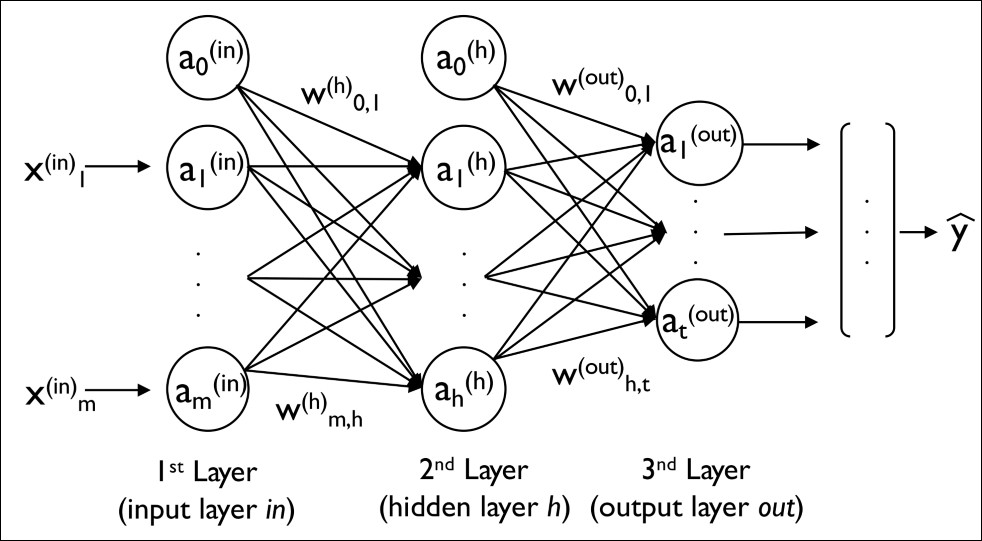
\includegraphics[width=0.6\columnwidth]{figures/MLP.jpeg}
        % note that in above figure file name, "sr_setup",
        % the file extension is missing. LaTeX is smart enough to find
        % apropriate one (i.e. pdf, png, etc.)
        % You can add this extention yourself as it seen below
        % both notations are correct but above has more flexibility
        %\includegraphics[width=1.0\columnwidth]{sr_setup.pdf}
        \caption{
                \label{fig:mlp} % spaces are big no-no withing labels
                % things like fig: are optional in the label but it helps
                % to orient yourself when you have multiple figures,
                % equations and tables
                An example of a MLP, taken from \cite{newmlp}. In this example, predictions $\hat{y}$ are generated from inputs $x^{(in)}$ using artificial neurons $a$ and weights $w$.
        }
\end{figure}

Whilst it is possible to train these MLPs with the Hillas parameters for a set of IACT images (though they tend to be inferior classifiers to BDT methods due to the fact that they don't prioritise parameters based on separation power \cite{hessbdt}), 
using every pixel value of an image as an input to an MLP tends to be computationally prohibitive.

\subsection{Loss Functions and Metrics}
\label{MLdefs}
In order to train a neural network, one needs to define a loss function for the training algorithm to optimise against. For binary, two class classification, the appropriate choice for this is the  binary cross entropy (BE) between the actual known classes $t_i$ and the score assigned by the network for an event having that class $s_i$ \cite{Keras}. This is defined over $N$ events as
\begin{equation}
    \textrm{BE}=-\frac{1}{N}\sum_{i=1}^{N}t_i\ln{s_i}+(1-t_i)\ln{(1-s_i)}.
\end{equation}

For multi-class (>2) classification the most appropriate choice is a \textbf{Categorical Cross-Entropy Loss Function (CE)}. This is defined \cite{Keras} as :
\begin{equation}
    \textrm{CE}=-\sum_i^N \ln \left( \frac{e^{t_{i}}}{\sum_j^3 e^{s_{ij}}} \right)
\end{equation}

where there are N events, $s_{ij}$  is the CNN score for each of the possible event classes for the event $i$ and $t_{i}$ is the CNN score for the target (true) class for that event. This equation relies on the CNN input labels being `one-hot' encoded such that the label for class $0$ is represented as $[1,0,...]$, class $1$ as $[0,1,...]$ so on \cite{fb}. In practice, during the training of the ConvLSTM2D networks in Chapters \ref{ch:3-TimingInfo} and \ref{ch:4-VERITASRealData}, there is an additional regularization penalty added to the total loss used due to the L2 regularization we use in the first two ConvLSTM2D layers. This regularization is designed to prevent network weights from taking extreme values.

\begin{table}[ht]
    \centering
    \resizebox{0.7\textwidth}{!}{
    \begin{tabular}{c|c}
    \textbf{Term} & \textbf{Definition}\\
    \hline
    \textbf{True Positive (TP)} & True Label Positive and Classification Positive\\
    \textbf{True Negative (TN)} & True Label Negative and Classification Negative\\
    \textbf{False Positive (FP)} & True Label Negative and Classified Positive\\
    \textbf{False Negative (FN)}& True Label Positive and Classified Negative\\
    \end{tabular}  
    }
    \caption{Definitions of Event Classifications for binary classification, taken from \cite{fawcett}.}
    \label{table:FPR}
\end{table}

For the purposes of evaluation of network performance, \textbf{Categorical Accuracy} \cite{Keras} is defined as the percentage of events for which the \textit{Argmax} of the one-hot-encoded predicted label is the same as the \textit{Argmax} for the one-hot-encoded true label (the definition of binary accuracy is similar for 2-class classification \cite{Keras}). Given the definitions for binary classification in Table \ref{table:FPR}, the \textbf{True Positive Rate (TPR)} and \textbf{False Negative Rate (FNR)} are defined by \cite{fawcett}:
\begin{equation}
    TPR=\sum_{Events}\frac{TP}{TP+FN}=1-FNR
\end{equation}
and the \textbf{True Negative Rate (TNR)} and \textbf{False Positive Rate (FPR)} by
\begin{equation}
    TNR=\sum_{Events}\frac{TN}{TN+FP}=1-FPR.
\end{equation} For multi-class ($>2$ class) classification, such as in Chapter \ref{ch:3-TimingInfo}, we use a one-versus-all approach where for each individual class the classifications are treated in a binary way (such as $\gamma$-ray or not-$\gamma$-ray) \cite{fawcett}\cite{scikit}. 

\subsection{Universal Approximation Theory}
Universal functional theory states that a neural network can be made to replicate the behaviour of any function, provided sufficient training data exists. However in practice this is limited by finite training data, a finite number of neurons in a layer, and a finite number of layers \cite{universal}. Ultimately through training for IACT event classification, it is such a function that we wish CNN-based classifiers to replicate, mapping a set of input images to an output event score. 

\subsection{Activation Functions}

The summed inputs to an artificial neuron are evaluated against activation functions. This is crucial to neural networks being able to solve highly non-linear problems such as the EXOR problem \cite{universal}. In particular, the final layer activation function in a neural network determines the form of the neural network output. The precise mathematical form of the activation function used by the neuron is a choice for the user; the earliest neural networks used simple Heaviside Step functions, but 
it is common to use Linear Rectifier (ReLU), $\tanh$ ($\sigma_T$) or sigmoid ($\sigma_S$) functions as they are useful for analysing nonlinear relationships \cite{C++CNN} \cite{Keras}. 

The Linear Rectifier Function ($\textrm{ReLu}(x)$) as a function of input variable $x$ as a function of threshold variable $y$ (typically 0, but configurable) is defined by
\begin{equation}
    \textrm{ReLu}(x)=\begin{cases}\mbox{0} & \mbox{, if } x <= y \\ \mbox{x} & \mbox{, otherwise} \end{cases}
\end{equation}

\cite{Keras}. The Sigmoid function ($\sigma(x)$), appropriate as the final layer activation function for binary classification. It takes the form

\begin{equation}
    \sigma(x)=\frac{1}{1+\exp(-x)}
\end{equation}

The Softmax function is a generalization of the Sigmoid function, and is appropriate as the final layer activation function for multi-class (>2 class) classification. For a vector input $(\textbf{x})$ with $i$th components $x_i $ and a given number of classes $K$ it is defined as
\begin{equation}
    \sigma(\textbf{x})_i=\frac{e^{x_i}}{\sum_{j=1}^K e^{x_j}}
\end{equation}

Neural networks can also be used as a method for regression, by having training data with continuous labels and modifying the activation function of the final layer in the network to provide a score on a continuous space. This can be used for IACTs for directional and energy reconstruction, however this thesis doesn't approach this issue (further information can be found for example in \cite{mikaelphd} and \cite{tjarkicrc}).  

\subsection{Convolutional Neural Networks}
Convolutional Neural Networks (CNNs) are a type of neural network developed specifically to handle image data, inspired by the mechanics of the visual cortex in the brain. Although the concept of a CNN dates back to 1980 (the so called neocognitron \cite{neocongnitron}), the first modern use of this taking advantage of GPU power was in a paper by Ciregan et.al. in 2012 \cite{ciregan}. CNNs take advantage of two properties of images, the translational invariance of useful data in the image (i.e. in Figure \ref{fig:carnet} it doesn't matter where in the image the car is located for the image to be classified as containing a car) and the relative sparsity of useful information in the image (i.e. the network does not need a million pixels to detect the presence of a tyre). The CNN achieves this in a `convolutional layer' by only feeding a few neighbouring pixels (a so-called receptive field) into each neuron, which are arranged in a 2D grid. The weights of these neurons are then shared throughout the convolutional layer in order to achieve the effect of translational invariance. Through pooling, downsampling and flattening, 
these neurons feed into MLP-like layers at the end of the network to perform a classification. CNNs are a promising technology for CTA analysis, as the entirety of the information contained in an IACT image can be used.  Another key advantage such CNN-based methods is the speed at which they can perform classifications of complete images (approximately 1kHz for Mono-telescope analysis using a NVidia 1080Ti GPU), which is a major factor to consider given the high expected array trigger rate of CTA (approximately $\mathrm{10\,kHz}$ for a full CTA array [56], although this estimate requires updating for the 'alpha' array configuration).

\begin{figure}[t!] 
        % read manual to see what [ht] means and for other possible options
        \centering 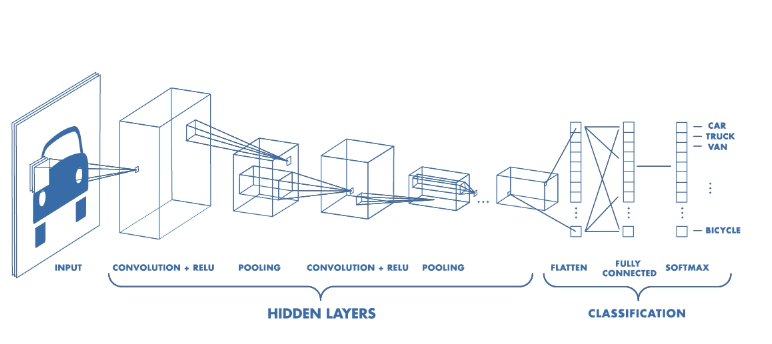
\includegraphics[width=1.0\columnwidth]{figures/carnet.png}
        % note that in above figure file name, "sr_setup",
        % the file extension is missing. LaTeX is smart enough to find
        % apropriate one (i.e. pdf, png, etc.)
        % You can add this extention yourself as it seen below
        % both notations are correct but above has more flexibility
        %\includegraphics[width=1.0\columnwidth]{sr_setup.pdf}
        \caption{
                \label{fig:carnet} % spaces are big no-no withing labels
                % things like fig: are optional in the label but it helps
                % to orient yourself when you have multiple figures,
                % equations and tables
                An example of a CNN, taken from \cite{mathworks}. Images are fed into convolutional layers, the outputs of which are flattened and fed into a MLP-like network prior to the output layer. Increasing the number of layers (depth) of the network increases the abstraction of the features recognised.
        }
\end{figure}
\subsection{Long Short-Term Memory Networks and ConvLSTMs}

Long Short-Term Memory networks (LSTMs) are are an established form of neural networks for time series analysis (which are more generally known as Recurrent Neural Networks or RNNs). They are heavily used in industry for classification tasks which require the ability to handle input vectors of varying length and having varying time intervals between useful information. A classic example of such a task is speech recognition.
LSTMs are mathematically similar to MLPs, except that the neurons are arranged such that there are loops in the network architecture, and the individual cells within the network contain vectors $\textit{c}$ to act as a memory as well as a function to `forget' elements from that memory $\textit{f}$, an input function $\textit{i}(x)$ and an output function $\textit{o}$ that produces an output vector $O_t$ at a timestep $t$. The equations used in the initial paper on LSTMs define a forward pass through a cell \cite{Hochreiter} as
\begin{align}
\begin{split}
\textit{f}_t &= \sigma_s(W_{f} x_t + O_{f} h_{t-1} + b_f) \\
\textit{i}_t &= \sigma_s(W_{i} x_t + O_{i} h_{t-1} + b_i) \\
\textit{o}_t &= \sigma_s(W_{o} x_t + O_{o} h_{t-1} + b_o) \\
\textit{c}_t &= \textit{f}_t \circ c_{t-1} + \textit{i}_t \circ \sigma_t(W_{c} x_t + U_{c} O_{t-1} + b_c) \\
O_t &= o_t \circ \sigma_t(\textit{c}_t)
\end{split}
\end{align}
where $\circ$ is an element wise product, $U$ is an additional weight matrix, and finally $b$ are bias vectors which must be trained. It is also possible to combine the properties of LSTMs and CNNs together to form ConvLSTMs, the 2D versions of which are ideal for classifying time sequences of images from IACTs. These ConvLSTMs are similar in structure to conventional LSTMs, but their internal matrix operations are replaced by convolutional operations. 
\begin{figure}[ht] 
        % read manual to see what [ht] means and for other possible options
        \centering 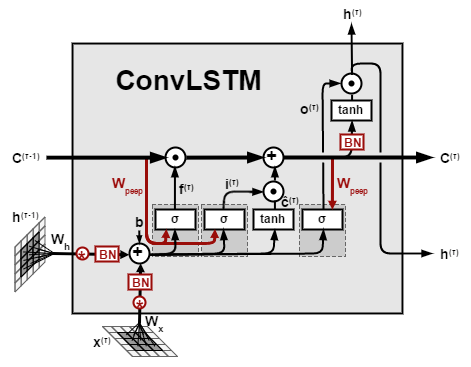
\includegraphics[width=0.5\columnwidth]{figures/convlstmcell.png}
        % note that in above figure file name, "sr_setup",
        % the file extension is missing. LaTeX is smart enough to find
        % apropriate one (i.e. pdf, png, etc.)
        % You can add this extention yourself as it seen below
        % both notations are correct but above has more flexibility
        %\includegraphics[width=1.0\columnwidth]{sr_setup.pdf}
        \caption{
                \label{fig:convlstmcell} % spaces are big no-no withing labels
                % things like fig: are optional in the label but it helps
                % to orient yourself when you have multiple figures,
                % equations and tables
                An illustration of the architecture of a ConvLSTM cell, taken from \cite{convlstmintro}.
        }
\end{figure}
A more detailed comparison between our ConvLSTM approach and the existing CRNN approach from Shilon et. al \cite{Shilon} can be found in Chapter \ref{ch:3-TimingInfo}.

LSTMs have now largely been supplanted by methods based on \textit{Attention} (a form of trainable weighted sum applied using fully connected dense layers in parallel) for most common time series analysis in industry. The \textit{CTLearn} \cite{tjarkicrc} CTA deep learning event reconstruction framework now offers a hybrid CNN/attention scheme, although the benefit of this for IACT analysis (compared to conventional CRNN methods) is currently unclear.

\subsection{Hyperparameters}
All machine learning algorithms (more complex than linear regression) have some number of hyperparameters, user-configurable options that define their architecture and the process of their optimisation. As examples, for a BDT or RF, this can be the number of trees in the classifier ensemble or the rate of `pruning' (the removal of branches from the trees), and for neural networks these can be the number of artificial neurons/convolutional filters per layer. Deep learning analyses innately require a greater number of hyperparameters than their conventional counterparts \cite{hyperopt}. Setting the values for these hyperparameters has typically been something of a dark art, although automated methods for determining hyperparameters have been developed \cite{hyperopt}. We explore this further in chapters \ref{ch:3-TimingInfo} and \ref{ch:4-VERITASRealData}.

\subsection{Weight Optimisation Algorithms}
The choice of weight optimiser used during training is also an example of a hyperparameter. Various algorithms exist to optimise the weights in a neural network during training. In Chapter \ref{ch:3-TimingInfo} we use the Adadelta algorithm to optimise our ConvLSTM2Ds as this was the \textit{Keras} recommended choice \cite{adadelta}, in Chapter \ref{ch:4-VERITASRealData} we found the Adam optimiser \cite{adam} performed marginally better.

Crucial to the performance of these algorithms is the concept of Backpropagation, which in effect allows the neural network optimiser to predict the effect of a change in a layer's weights by using the chain rule to compute a gradient (and therefore examine the effect of changing weights) in the loss function. Virtually all neural network optimisation algorithms use this technique \cite{goodfellow2016deep}.

\subsection{Over- and Under-training}
\begin{figure}[ht] 
        % read manual to see what [ht] means and for other possible options
        \centering 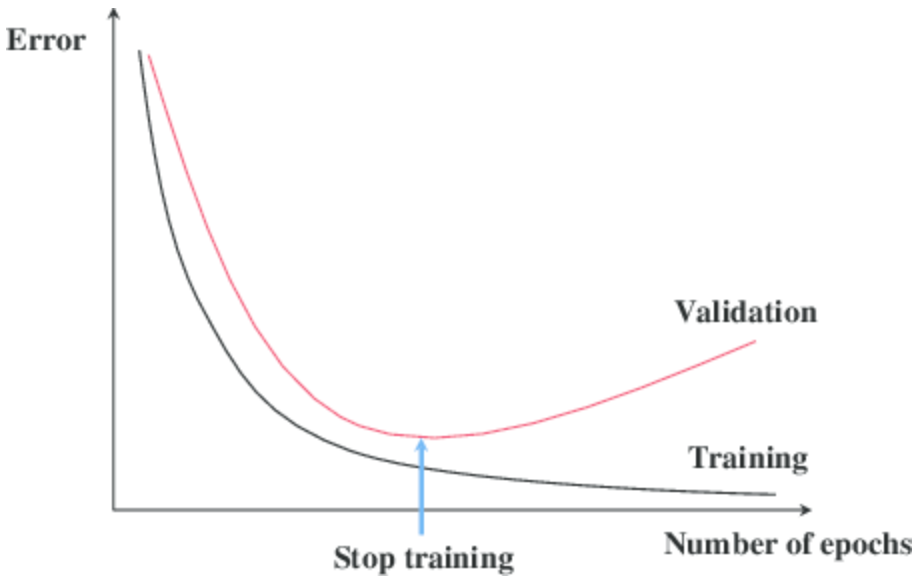
\includegraphics[width=0.7\columnwidth]{figures/overtrain.png}
        % note that in above figure file name, "sr_setup",
        % the file extension is missing. LaTeX is smart enough to find
        % apropriate one (i.e. pdf, png, etc.)
        % You can add this extention yourself as it seen below
        % both notations are correct but above has more flexibility
        %\includegraphics[width=1.0\columnwidth]{sr_setup.pdf}
        \caption{
                \label{fig:earlystop} % spaces are big no-no withing labels
                % things like fig: are optional in the label but it helps
                % to orient yourself when you have multiple figures,
                % equations and tables
                An illustration of the concept of over and under training, where error here can be considered equivalent to loss, taken from \cite{earlystop}, in practice we found the use of validation data to be unreliable and highly noisy.
        }
\end{figure}

Neural networks can be both over- and under- optimised during the training process, a feature illustrated in Figure \ref{fig:earlystop}. One option to prevent this is to define an early stopping condition, whereby training is abandoned and the weights in a network reverted to those from a previous epoch, though this depends on both reliable validation performance and the ability to define a suitable metric by which to stop training. We encounter such issues in Chapter \ref{ch:3-TimingInfo}.


\subsection{Dropout and Regularization}
Dropout refers to a procedure during training of randomly setting weights in the network to zero, at a configurable rate. This is an extremely common practice in deep learning and is designed to prevent overtraining of networks. Typically, the dropped out weights are frozen after training, but applying dropout during testing can be used as a method of pseudo-simulating Bayesian posteriors \cite{mike}\cite{gal2015}. 

Regularization is a similar technique whereby additional bias terms are introduced to neural network loss functions to penalize overly-large weights, and thus also prevent overtraining. In this work, we use L2 regularization whereby a quantity ($L2$) defined by
\begin{equation}
    L2=\lambda\sum_{i}w_i^2
\end{equation}
, where $\lambda$ is a configurable hyperparameter and $w_i$ are the network weights, is added to the loss function \cite{Keras}.

In the \textit{Keras} \cite{Keras} package, dropout and regularization can be applied to the CNN elements of a network (Kernel Dropout and Regularization) or the Recurrent elements of a network (Recurrent Dropout and Regularization) or both; the rate and $\lambda$ terms of both being configurable hyperparameters.

\section{Past and Concurrent Work on CNN Use With IACT data}
In this section, we review recent relevant work concerning the use of these new machine learning methods for IACTs.

\subsection{Muon Tagging and Muon-Hunters}
The first published work to consider the potential for CNN-type analysis with IACTs was Feng et.al in 2016 \cite{feng2016}. The authors consider the use of CNNs for muon ring classification (selecting events where a muon has passed directly down the optical path of an IACT and has therefore produced a characteristic 'ring' image) as well as muon ring radius and size regression with VERITAS. This is needed for online calibation, as by measuring the width and detected Cherenkov light intensity of such events, one can infer the efficiency of the IACT's optics. VERITAS has also investigated the use of active learning for the same purpose through the Muon Hunters 2.0 project \cite{muonhunters2}, whereby classifications from citizen scientists are used in combination with Bayesian deep learning to improve classifications.

Whilst active-learning is an extremely interesting area of computer science research, and an excellent opportunity to engage the public, the task of gamma/hadron separation for CTA is less well suited for active-learning-type analyses for a number of reasons. Firstly, the likely trigger rates (10kHz) \cite{trigrate} of CTA are probably beyond the reasonable capacity of an active-learning pipeline, as the number of citizen scientist volunteers over time is usually approximately constant. Secondly, current active-learning analyses can have significant biases inherited from the intuition of volunteers (such as the redshift dependence on galaxy morphology classification in \cite{mike}), that are probably currently intolerable for high level scientific analysis to be reliably performed. Thirdly, gamma/hadron separation for IACTs is both a subtle (relying on small differences between images and therefore difficult for humans to perform) and uninteresting task. There are likely no exciting discoveries, equivalent to new types of galaxy or new planets, for citizen scientist volunteers to make in IACT event classification images that could not be simply detected in IACT data by (for example) selecting the brightest (highest energy) events. Finally, as these methods ultimately rely upon CNNs, they are vulnerable to the same run-by-run experimental variations as supervised deep learning techniques. We discuss these issues later Chapter \ref{ch:4-VERITASRealData}. As such, in our opinion, supervised machine learning methods remain the most promising for IACT event classification for CTA.

R. Clark has also recently studied further potential options for muon tagging with CHEC-S and ASTRI simulated data using CNNs \cite{roganthesis}, particularly concerning the tagging of partial muon rings against proton EAS background. Whilst he found that CNNs can identify partial muon rings (despite the complexity of generating a simulated dataset suitable for this analysis), it appears as if using supervised CNNs for online muon tagging will suffer many of the same issues surrounding CNN use for IACT background rejection that we explore further in Chapter \ref{ch:4-VERITASRealData}.

\subsection{Work of Shilon et al. and Parsons et al.}
Shilon et al. \cite{Shilon} and Parsons et al. \cite{ParsonsOhm} are the two papers currently in press that concern the application of deep learning event classification and reconstruction methods to H.E.S.S. data. Whilst these have provided significant advances in the field (particularly in the case of the Shilon et al. work), there are a number of underlying issues that have become apparent since their publication.

In the Shilon et al. work \cite{Shilon}, the authors feed images from the CT1-4 telescopes into convolutional layers that then feed into an LSTM Network. This technique, the authors call the Convolutional Recurrent Neural Network (CRNN) method, treats the set of four charge images from the four IACTs as a time series. The authors of the Shilon et al. work justify this network architecture using the assumption that that the images with the largest size parameter (total charge) are those closest to the shower core, and that this ordering compensates for the lack of available temporal information in their case \cite{Shilon}. Using this, they observed performance in background rejection superior to the current BDT paradigm with simulations, and were able to perform a significant detection of PKS 2155-304 with real observations. The CRNN technique achieved a $\mathrm{50.8\,\sigma}$ detection with this data relative to a BDT which achieved $\mathrm{46.1\,\sigma}$, though the statistical significance of this difference has not been completely explored. In particular, this source is extremely bright, and so this data is likely $\gamma$-dominated. Whilst this network architecture allowed for the first CNN-based detection of an astrophysical source, the Shilon et al. work's authors' assumption that the ordering of the images in the LSTM is significant has not necessarily held up to subsequent scrutiny, with other charge image orderings \cite{ariconf} being seen to provide equivalent or superior performance. As a result, for the purposes of our work in later chapters, we treat the LSTM-type features in similar networks as a computational tool. Whilst this tool is useful for avoiding the need to stack images from multiple telescopes into single images in order to apply CNN-type analyses (which had been the standard previous to the Shilon et al. work and doesn't scale well in the case of multiple IACTs \cite{Shilon} \cite{salvatore} as details in images from high multiplicity events is lost), we ultimately don't assume the use of the LSTM features in such networks to be of further physical significance in later chapters. Additionally, the Shilon et al. paper considers directional reconstruction, however the directional and gamma/hadron separation elements of the paper are applied to differing flaring states of PKS2155-304, suggesting significant issues with applying stereoscopic directional reconstruction methods to real observations. The most likely cause of this is a lack of an appropriate pointing correction algorithm for CNN-type analysis, and the difficulty of taking appropriate account of IACT positions on the ground. The later Parsons et al. \cite{ParsonsOhm} work attempts to hybridise CNN-type methods with parametric inputs such as impact parameters for background rejection, however this partially defeats part of the point of using whole-image CNN methods. Ideally, the aim is to get the CNN classifier to learn image features related to (for example) impact distance from the images themselves. It is also not at all clear in that paper the relative contributions of the image and parametric network components to the event classification, a parametric MLP with the same parameterised data would likely perform as well as the hybridised CNN approach. It is not currently clear how well these CNN-based event classification methods will work with dimmer sources given their high level of sensitivity to small differences between real observations and simulations. We explore such issues related to real observations further in Chapter \ref{ch:4-VERITASRealData}.

One critical issue that both the Shilon et al. and Parsons et al. paper share is their reliance on tailcut cleaning of images prior to deep learning analysis. For example, see the following quote from the Shilon et al. paper:
\begin{quote}
    \textit{The raw simulated images are cleaned according to the standard H.E.S.S. cleaning scheme.}
\end{quote}

The complication from this is that if the aim of deep-learning-based event classification methods on photomultiplier charge data is to improve sensitivity to subtle features in IACT images, tailcut cleaning will make analysis of real observations simpler (as only a handful of pixels' noise needs to be accurately modelled rather than several hundred), but will remove the features in the images we aim to exploit. Whilst this can be argued as being a necessary constraint of a proof-of-concept study (common in many astronomy deep learning papers, see for example \cite{dodgygal}), in the long run if deep learning event classifiers cannot be performed without tailcut image cleaning they will never pass a cost/benefit analysis, and as such we should aim to find ways of avoiding the need to do so. That said, performing tailcut image cleaning before directional reconstruction is more tolerable, given that there is less need to examine small features around the edge of the shower image. We explore the limitations of performing charge-based deep learning event classification, without tailcut image cleaning, in Chapter \ref{ch:4-VERITASRealData}.  

\subsection{Full Event Reconstruction and Instrument Response Functions}
For most of the previous decade, a Python-based method of generating Effective Areas, Angular Resolution plots and Energy Sensitivities (examples of Instrument Response Functions (IRFs)) based on \textit{ctapipe} and the associated prototype pipelines did not exist. At the time of writing this is now only partially the case, and prototype methods of IRF generation have yet to undergo a full Monte-Carlo validation effort for either CHEC-S or SSTCAM. Much of the current work of the CTA task force on machine learning now focuses on generating these instrument response functions with deep learning classifiers, directional reconstructors and energy reconstructors \cite{tjarkicrc}. However, fundamentally the underlying task of CNN-based reconstruction has not changed, despite the ability to generate these new results. Additionally given the real observations issues explored in the next section, such IRFs generated using these pipelines likely have difficult to quantify systematic errors associated with the discrepancies between real and simulated data, as well as having issues with gammaness cut optimisation and asymmetric posteriors for gammaness \cite{mike}. As such, IRFs based on deep learning analyses pipelines may well be unreliable in practice for the foreseeable future. We explore these issues in depth in later chapters.

\subsection{Multi-Task Learning}

One option is to design a CNN-based architecture to perform the tasks of event classification, directional reconstruction and energy reconstruction simultaneously, work currently being done by the \textit{Gammalearn} project \cite{mikaelphd} (primarily for single telescope analysis). The motivation for this is that there are physical correlations between the event impact distance and apparent energy. Whilst a very interesting area of investigation, attempting to perform multiple IACT analysis tasks simultaneously makes it difficult in practice to discern where any improvement in performance originates from, and it also makes the implicit assumption that the optimal simulation and analysis setup is the same for Event Classification, Directional Reconstruction and Energy Reconstruction. This is not mandated to be the case, in all likelihood given the existence of ImPACT, the main potential benefit from deep-learning-based directional reconstruction is speed, whereas for gamma-hadron separation the main goal is likely to be sensitivity. Similarly, applying tailcut cleaning for $\gamma$/hadron separation with deep learning classifiers largely defeats the purpose of using whole image analysis, whereas tailcut cleaning for directional reconstruction is more likely to be tolerable (and will help against NSB) since there is less dependence on minute features near the shower image edge. That said, the clear sensitivity of CNNs to event direction we find in Chapter \ref{ch:3-TimingInfo} suggests there may be a significant benefit to performing event classification and directional reconstruction simultaneously.

\section{Known Issues with CNN-Type Analysis Techniques}
In the following subsections we discuss the various known issues associated with the use of CNNs for CTA analysis. It is helpful to define problems when exploring new analysis methods as it helps in the process of defining goals and limitations. This is particularly true in the case of CTA, as it consists of a new set of instruments with new procedures and analysis requirements,

\subsection{The Camera Geometry Problem}

Firstly, CNNs are primarily designed to process square images. This creates an issue for using CNNs with CTA data as many of the camera prototypes have focal planes which are either hexagonal or have regions without photodetectors (like CHEC, which doesn't have photodetectors in its corners). In the case of hexagonal cameras, there are two options to avoid the risk of geometric bias. The first is to resample or oversample the hexagonal image in order to make it square, this is the approach taken in a paper by Holch et.al. \cite{Hexagdly} and used in Chapter \ref{ch:4-VERITASRealData} for our VERITAS data. The second option is to write a custom CNN code that can handle hexagonal images based on computing convolutions based on nearest neighbour information, which may also be applicable to CHEC/SSTCAM (in the analysis in Chapter \ref{ch:3-TimingInfo} we just crop images to the square central region of the camera). The disadvantage of this custom CNN approach is that it limits the potential for more sophisticated network architectures, and at present has not been extended to stereoscopic analysis. Graph-based Chebyshev networks \cite{adithesis} might provide an alternative solution to this problem in the long term, as they only require that an adjacency matrix can be defined for the camera plane, as opposed to having to perform transformations to place the IACT images on a Euclidean grid. 

\subsection{The Multiple Telescope Problem}

CTA will operate stereoscopically, and combining images from multiple telescopes (separated by varying distances on the ground and differing impact distances) to use with CNNs is a problem unique to IACTs. The simplest method of solving this problem used by many IACT researchers is to simply add the pixel values from the various telescopes together and feed this single image to a CNN \cite{mangano}. The problem with this is that it doesn't take account of the telescopes' positions on the ground, which is an issue for performing accurate reconstruction. It also doesn't scale well to large arrays; if only five telescopes are triggered in an array of a hundred, the resulting stacked images are very sparse (a problem for CNNs). This is complicated further by CTA's multiple classes of telescope.

Over the course of the investigations included in chapters \ref{ch:3-TimingInfo} and \ref{ch:4-VERITASRealData}, it has become apparent that there will likely always be some degree of tension between the most advanced deep learning analyses possible and stereoscopic IACT analysis. This is as single image analysis is both a more common task and is easier to perform.  However it is important to note that stereoscopic analysis for IACTs basically always achieves superior sensitivity and event angular resolution against single image analysis with any analysis method, as the pixel density and effective area of a single IACT is limited by technological constraints. As such, if deep learning analysis cannot eventually work on images from multiple IACTs, it's worth is reduced in the context of an advanced analysis method for CTA.

As of the time of writing, no CTA deep learning analysis study has seriously considered the prospect of deep learning event classification with multiple classes of CTA telescope observing the same event. This may be one of the must crucial avenues of investigation given the flexibility deep learning offers in considering partially truncated shower images. However, investigating this comes with significant computational cost and simulation complexity.

\subsection{The Hyperparameter Problem}
CNN-type methods require a large number of hyperparameters, which aren't trivial to human-interpret. The optimal combinations of these for IACT data may be a function of instrument observational energy, plate scale and observation conditions, and automated optimisation strategies for these are highly computationally costly. Additionally hyperparameter selection can have an effect on training convergence, which makes comparison of differing models complex. We explore these issues in depth in Chapter \ref{ch:4-VERITASRealData}.

\subsection{The Real Observation Problem}
Whilst one of their greatest strengths, the fact that CNNs are sensitive to minute morphological features in their training datasets can also present significant issues. The most troublesome problem arises from the fact that we need a labeled input dataset in order to train our networks. In certain cases (such as transient searches \cite{SNH}) this dataset can be produced from real observations by hand, or through the involvement of citizen scientists. However, for the purpose of CTA image analysis this is not possible. As a result, we are forced to train our neural networks on data simulated using Monte-Carlo simulations for which we know the `true' event parameters, and then use these trained networks to analyse real observations. The slightest discrepancy between the real and simulated data (for example from night sky background, optical efficiency losses due to the ageing of the telescopes or imperfect calibration) has the potential to affect the resulting analysis. One particular source of concern for the CTA SSTs in particular is the uncertainty in modelling hadronic processes at high energies (notably in the CTA standard \textit{Quark Gluon String with JETs (QGSJet)} package used by \textit{CORSIKA}), due to a lack of forward momentum data from the LHC. Significant work to improve these models is nonetheless underway \cite{hadronmodel}.

One potential solution to this problem has been proposed by Erdmann et.al. \cite{ErdmannAuger}. Their suggestion is the use of Generative Adversarial Networks, which are essentially two CNNs playing off each other in a zero sum game \cite{goodfellow2016deep}, to perform an intelligent, machine learning based correction to simulated data such that it resembles real observations more closely for the purpose of training a CNN. We briefly further discuss the potential applications of GANs in Chapters \ref{ch:3-TimingInfo} and \ref{ch6-Conclusions}.

\subsection{The Class Imbalance Problem}

Not every $\gamma$-ray source on the sky is equally bright, and so real test data will typically be imbalanced (i.e. not have a 50:50 $\gamma$ to proton ratio). In certain IACT use cases, such as obtaining dark matter annihilation constraints from observations of dwarf spheroidal galaxies (such as \cite{gloryduck}), the observational data will be proton dominated. In particular, this is complicated by trigger selection. As a result, there is a need for a future detailed investigation into the effects of using more realistic, imbalanced training data with CNN-type IACT background rejection methods, as such imbalanced datasets require specialised deep learning treatments \cite{imbalance}.

\subsection{The GPU Cost and Availability Problem}
Without access to high-performance GPUs, deep learning analysis would be prohibitively slow as an analysis method for CTA, at both training and inference times. Whilst extremely powerful computational tools, GPUs are very expensive \cite{gpucost}, in very short supply \cite{gpushort}, power hungry \cite{2080ti} and thus costly to run \cite{2080ti}. These practical considerations must be taken into account when considering deep learning as a potential general analysis method for CTA. In the long term, and broadly speaking for the majority of analyses, deep learning analysis must have a reasonable prospect of passing a cost/benefit analysis whereby if deep learning offers a 10\% improvement in sensitivity, it must be less than 10\% more computationally and financially costly compared to conventional analysis. At the time of writing, this is not the case, however there could be specific analysis cases where such costly analysis methods could be justified if it opens the potential for new physics (such as looking for dark matter annihilation constraints through observing dwarf spheroidal galaxies\cite{gloryduck}).

Given these issues of availability and cost, there is a serious risk of deep-learning-based research in the physical sciences becoming a `walled garden', whereby only the richest or most cited researchers have access to sufficient compute power to perform state-of-the-art deep learning analyses \cite{gpudivide}. Ideally, GPU time should be allocated based on scientific merit, and to their credit the UK's Science and Technology Facilities Council (STFC) are now providing such a peer reviewed resource through their eInfrastructure for Research and Innovation for STFC (IRIS) scheme, now being utilised by CTA.